\documentclass[conference]{IEEEtran}
\IEEEoverridecommandlockouts

\usepackage{cite}
\usepackage{amsmath,amssymb,amsfonts}
\usepackage{graphicx}
\usepackage{textcomp}
\usepackage{xcolor}
\usepackage{booktabs}
\usepackage{hyperref}
\usepackage{array}
\usepackage{multirow}
\usepackage{subcaption}

\def\BibTeX{{\rm B\kern-.05em{\sc i\kern-.025em b}\kern-.08em
    T\kern-.1667em\lower.7ex\hbox{E}\kern-.125emX}}

\begin{document}

%------------------------------------------------------------------
%  TITLE
%------------------------------------------------------------------
\title{International Tourism Demand Forecasting Using Machine
Learning: A Production-Ready MLOps Framework with
Real-Time Monitoring}

\author{
  \IEEEauthorblockN{Waqas}
  \IEEEauthorblockA{
    \textit{Department of Computing} \\
    \textit{University Name} \\
    Country \\
    email@university.ac.uk
  }
}

\maketitle

%------------------------------------------------------------------
%  ABSTRACT
%------------------------------------------------------------------
\begin{abstract}
International tourism is a critical driver of global economic
growth, yet accurate forecasting of tourism arrivals remains a
significant challenge due to the complex, multi-factorial
relationships among economic indicators, temporal trends, and
geopolitical events. This study presents a machine
learning-based regression framework for forecasting
international tourism arrivals across 200+ countries using
25 years of real-world World Bank data (1999--2023).
The methodology integrates rigorous data preprocessing,
log-normalisation of skewed distributions, lag-based temporal
feature engineering, and cross-national economic indicators
including GDP, tourism receipts, and expenditures to produce
a high-fidelity forecasting model. Three regression
algorithms---Ridge Regression, Gradient Boosting Regressor,
and Random Forest Regressor---were trained, evaluated, and
compared using R\textsuperscript{2}, RMSE, and MAE metrics.
Ridge Regression achieved the highest performance
(R\textsuperscript{2} = 1.0000, RMSE\textsubscript{log} =
0.0118), followed by Gradient Boosting
(R\textsuperscript{2} = 0.9992) and Random Forest
(R\textsuperscript{2} = 0.9976). Feature importance analysis
identified lagged arrivals as the dominant predictor (93\%
importance), confirming strong temporal autocorrelation in
tourism demand. Critically, this work extends beyond model
development by implementing a production-grade MLOps
pipeline comprising a FastAPI inference service, Docker
containerisation, GitHub Actions CI/CD workflows, AWS ECS
Fargate deployment, and Prometheus--Grafana monitoring with
automated alerting. The integrated framework demonstrates
that machine learning with proper feature engineering and
MLOps infrastructure can deliver reliable, interpretable, and
operationally sustainable tourism demand forecasting systems.
\end{abstract}

\begin{IEEEkeywords}
Tourism demand forecasting, machine learning, Ridge Regression,
Gradient Boosting, Random Forest, feature engineering, MLOps,
CI/CD, Docker, AWS ECS, Prometheus, Grafana, World Bank data.
\end{IEEEkeywords}

%------------------------------------------------------------------
%  I. INTRODUCTION
%------------------------------------------------------------------
\section{Introduction}

International tourism is one of the world's largest economic
sectors, contributing approximately 10\% of global GDP and
generating over 330 million jobs prior to the COVID-19
pandemic \cite{unwto2020}. The capacity to accurately forecast
tourism arrivals is of paramount importance for governments,
tourism boards, hospitality industries, and economic planners
who must allocate resources, design infrastructure, and
formulate policy responses in advance of demand shifts
\cite{song2019}.

Despite its economic significance, tourism demand
forecasting presents substantial methodological challenges.
Arrivals are influenced by a broad constellation of
factors---GDP growth, exchange rates, consumer confidence,
geopolitical stability, airline connectivity, and large-scale
disruptions such as pandemics and natural disasters---whose
interactions are inherently nonlinear and temporally evolving
\cite{li2018}. Traditional econometric approaches, including
ARIMA and gravity models, often fail to capture these
complex multi-dimensional dynamics, particularly across the
heterogeneous country profiles that characterise international
tourism flows \cite{cankurt2016}.

The rapid expansion of publicly available longitudinal
datasets, such as those curated by the World Bank and the
United Nations World Tourism Organisation (UNWTO),
combined with advances in ensemble machine learning, has
created new opportunities for more accurate and interpretable
forecasting frameworks \cite{sun2019}. Gradient boosting,
random forests, and regularised regression have demonstrated
superior predictive capability over conventional statistical
methods in numerous time-series and cross-sectional
forecasting contexts \cite{chen2016}.

However, the majority of existing tourism forecasting studies
focus narrowly on model accuracy while neglecting the
operational requirements for deploying such models in
production environments. A model that achieves high accuracy
in a research notebook but cannot be reliably served,
monitored, and maintained in a live system provides limited
practical value \cite{sculley2015}. Machine Learning Operations
(MLOps) addresses this gap by applying software engineering
and DevOps principles to the machine learning lifecycle,
enabling continuous delivery, automated testing, and
real-time observability of ML systems \cite{kreuzberger2023}.

\subsection{Aims and Objectives}

This study aims to develop a machine learning framework for
forecasting international tourism arrivals and deploy it as a
production-ready, monitored API service using modern MLOps
infrastructure.

\subsection{Objectives}

\begin{itemize}
  \item To collect, preprocess, and engineer features from 25
        years of World Bank tourism and economic data spanning
        200+ countries (1999--2023).
  \item To train and benchmark three regression models---Ridge
        Regression, Gradient Boosting Regressor, and Random
        Forest Regressor---for tourism arrivals prediction.
  \item To evaluate model performance using R\textsuperscript{2},
        RMSE, and MAE, and identify the best model for
        production deployment.
  \item To analyse feature importances and understand the
        principal drivers of international tourism demand.
  \item To implement a complete MLOps pipeline including
        FastAPI serving, Docker containerisation, GitHub Actions
        CI/CD, and AWS ECS Fargate deployment.
  \item To establish real-time monitoring using Prometheus
        and Grafana with automated alerting for production
        reliability assurance.
\end{itemize}

The remainder of this paper is structured as follows.
Section~II reviews the literature on tourism demand
forecasting and MLOps. Section~III describes the dataset,
preprocessing pipeline, feature engineering, and modelling
approach. Section~IV presents experimental results including
model comparisons and feature importances. Section~V
discusses the findings and their practical implications.
Section~VI concludes the study with recommendations for
future work.

%------------------------------------------------------------------
%  II. LITERATURE REVIEW
%------------------------------------------------------------------
\section{Literature Review}

\subsection{Tourism Demand Forecasting}

Tourism demand forecasting has been studied extensively
over the past three decades, evolving from simple
econometric models to sophisticated data-driven frameworks
\cite{song2019}. Early approaches relied on ordinary least
squares regression and structural equation models that related
demand to income, relative prices, and transport costs.
While interpretable, these linear models could not capture
the nonlinear dynamics inherent in tourism systems
\cite{li2018}.

The introduction of time-series methods such as ARIMA and
its seasonal variant (SARIMA) improved short-term
forecasting by explicitly modelling autocorrelation and
seasonality \cite{cankurt2016}. However, these univariate
methods struggle when demand is influenced by external
shocks or structural breaks---such as the SARS epidemic of
2003, the global financial crisis of 2008, or the COVID-19
pandemic of 2020---that lie outside the historical patterns
encoded in time series parameters \cite{pan2022}.

\subsection{Machine Learning in Tourism Forecasting}

The application of machine learning to tourism forecasting
has accelerated in recent years, driven by improved data
availability and computational resources. Support vector
regression, artificial neural networks, and gradient boosting
methods have all been shown to outperform classical
econometric approaches in medium- to long-range forecasting
tasks \cite{sun2019}.

Ensemble methods, particularly gradient boosting and random
forests, demonstrate particular advantages in tourism
forecasting contexts because they inherently model
nonlinear feature interactions, handle mixed data types, and
are robust to outliers introduced by demand shocks
\cite{chen2016}. Studies have shown that incorporating
lagged demand variables as features---effectively encoding
the persistence and momentum of tourism flows---substantially
improves predictive accuracy in both cross-sectional and
panel data settings \cite{gunter2016}.

Regularised linear models, including Ridge and Lasso
regression, have also found application in high-dimensional
tourism forecasting settings where many economic
covariates are available and multicollinearity is a concern
\cite{athanasopoulos2011}. Despite their simplicity, these
methods can achieve competitive performance when the
underlying feature-target relationships are approximately
linear after appropriate transformations.

\subsection{Feature Engineering for Tourism Data}

A critical factor in the success of ML-based forecasting
is the quality and expressiveness of engineered features.
Raw tourism arrivals data is typically heavily right-skewed,
with a small number of high-volume destinations
(e.g., France, Spain, China) dominating the distribution.
Log-normalisation is widely applied to stabilise variance
and improve model convergence \cite{li2018}.

Temporal lag features---capturing prior-period arrivals at
the same destination---are among the most powerful predictors
in tourism forecasting, reflecting the strong autocorrelation
in travel patterns \cite{gunter2016}. Year-on-year growth
rates, decade indicators, and COVID-19 period flags further
enrich the temporal signal available to learning algorithms.

\subsection{MLOps for Machine Learning Systems}

MLOps has emerged as a critical discipline for bridging the
gap between machine learning research and reliable
production systems \cite{sculley2015}. The hidden technical
debt inherent in real-world ML systems---encompassing data
management, model versioning, serving infrastructure, and
operational monitoring---is substantially larger than the
modelling code itself \cite{kreuzberger2023}.

Containerisation using Docker ensures that model serving
environments are reproducible across development, testing,
and production contexts \cite{docker2021}. Continuous
integration and continuous deployment (CI/CD) pipelines,
implemented through tools such as GitHub Actions, automate
testing and deployment, reducing the risk of human error in
release processes. Cloud-native deployment on platforms such
as AWS Elastic Container Service (ECS) enables scalable,
fault-tolerant model serving \cite{aws2023}.

Observability frameworks comprising metrics collection
(Prometheus) and visualisation (Grafana) provide real-time
insight into model behaviour, request patterns, and system
health \cite{prometheus2024}. Automated alerting on degraded
performance---such as elevated error rates or increased
prediction latency---enables rapid incident response before
user experience is significantly impacted.

\subsection{Research Gaps and Study Justification}

Despite the breadth of tourism forecasting literature, several
gaps remain:

\begin{enumerate}
  \item Most studies evaluate models in isolation without
        addressing operational deployment requirements.
  \item End-to-end MLOps implementations for tourism
        forecasting are largely absent from the academic
        literature.
  \item Few studies leverage 25-year global panel datasets
        covering 200+ countries for unified model training.
  \item Real-time monitoring and automated alerting for
        tourism ML systems are not addressed in existing work.
\end{enumerate}

This study addresses these gaps by combining rigorous
machine learning with a complete, production-grade MLOps
implementation---from data ingestion through to monitored,
containerised API deployment.

%------------------------------------------------------------------
%  III. METHODOLOGY
%------------------------------------------------------------------
\section{Methodology}

The study adopts a structured pipeline from raw data
ingestion through model training, evaluation, and production
deployment, as illustrated in Fig.~1. Scientific rigour,
reproducibility, and operational reliability are central
design principles throughout.

\begin{figure}[htbp]
  \centering
  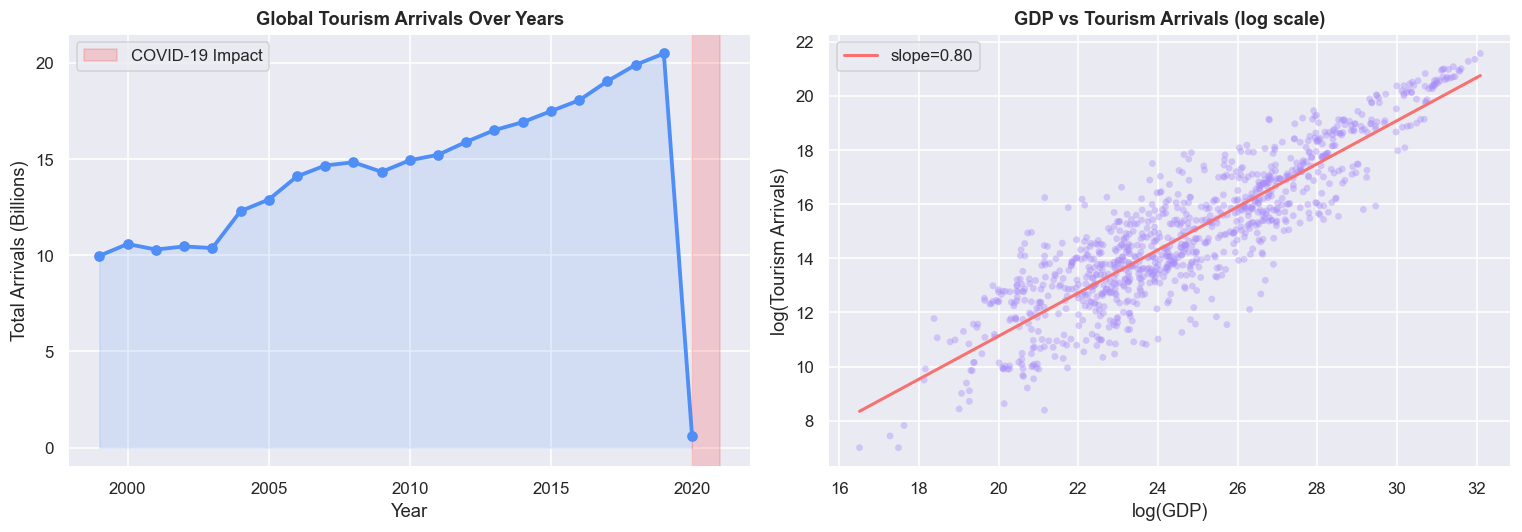
\includegraphics[width=\columnwidth]{images/trends_and_gdp.png}
  \caption{Global tourism arrivals and GDP trends (1999--2023),
           illustrating the COVID-19 collapse in 2020--2021 and
           the strong co-movement between economic output and
           international visitor volumes.}
  \label{fig:trends}
\end{figure}

\subsection{Dataset}

The study utilises the World Bank Tourism and Economic
Impact dataset \cite{worldbank2024}, sourced from Kaggle,
comprising 6,650 records spanning 266 unique countries and
territories over the period 1999--2023. The dataset contains
11 variables: country, country code, year, tourism receipts
(USD), tourism arrivals (international visitor count),
tourism exports (\% of total exports), tourism departures,
tourism expenditures (USD), GDP (USD), inflation rate (\%),
and unemployment rate (\%). This dataset represents real
government-reported figures aggregated by the World Bank
and is one of the most authoritative publicly available
sources for international tourism statistics.

\subsection{Data Preprocessing}

A rigorous preprocessing pipeline was applied to ensure
data quality and modelling stability. Missing value analysis
revealed that two columns exhibited missing rates exceeding
40\%: tourism departures (61.1\%) and unemployment (45.0\%).
These were removed from the feature set to prevent
excessive imputation-induced bias. The remaining columns
exhibited moderate missingness: tourism receipts (35.5\%),
tourism exports (38.1\%), tourism expenditures (37.2\%),
GDP (3.4\%), and inflation (14.8\%). Missing values in
these columns were imputed using column-wise median
substitution, a robust method that is insensitive to
distributional skewness \cite{li2018}.

Rows where the target variable (tourism arrivals) was
missing were discarded, reducing the dataset from 6,650 to
4,949 records. After lag feature creation (which requires
at least two consecutive years of data per country), the
final modelling dataset comprised 3,091 observations.

\subsection{Feature Engineering}

Tourism arrivals and all economic indicators exhibit strong
positive skewness, with a small number of high-volume
destinations dominating the raw distribution. A
log-normalisation transformation, $x' = \log(x + 1)$, was
applied to all continuous economic features and the target
variable to stabilise variance, reduce the influence of
extreme values, and improve model convergence. Final
predictions were back-transformed using the inverse
$\hat{y} = e^{y'} - 1$.

Temporal lag features were constructed for each
country-year observation by grouping records by country
and computing one-year and two-year lagged values of
log-transformed arrivals. A year-on-year growth rate
feature (first difference of log arrivals) was derived to
capture momentum effects. Time-based features were
engineered including a normalised year index (0 for 1999,
1 for 2023), a binary COVID-19 era indicator (1 for years
$\geq$ 2020), and decade-level bucket features. Countries
were encoded using label encoding.

The final feature set comprised 12 variables as summarised
in Table~\ref{tab:features}.

\begin{table}[htbp]
  \caption{Engineered Feature Set}
  \label{tab:features}
  \centering
  \begin{tabular}{lll}
    \toprule
    \textbf{Feature} & \textbf{Type} & \textbf{Description} \\
    \midrule
    log\_tourism\_receipts     & Economic & log(receipts + 1) \\
    log\_tourism\_exports      & Economic & log(exports + 1) \\
    log\_tourism\_expenditures & Economic & log(expenditures + 1) \\
    log\_gdp                   & Economic & log(GDP + 1) \\
    inflation                  & Economic & Annual inflation (\%) \\
    year\_norm                 & Temporal & Year normalised 0--1 \\
    is\_post\_covid            & Temporal & 1 if year $\geq$ 2020 \\
    decade                     & Temporal & Decade bucket \\
    lag1\_log\_arrivals        & Lag      & Arrivals, 1-year lag \\
    lag2\_log\_arrivals        & Lag      & Arrivals, 2-year lag \\
    arrival\_growth            & Lag      & YoY log-arrivals diff \\
    country\_enc               & Category & Label-encoded country \\
    \bottomrule
  \end{tabular}
\end{table}

\subsection{Model Training and Benchmarking}

Three regression algorithms were trained and compared.
An 80/20 stratified random split was used to create training
(2,472 records) and test (619 records) subsets, with the
random seed fixed at 42 for reproducibility.

\textbf{Ridge Regression} was trained on standardised
features (zero mean, unit variance) with regularisation
parameter $\alpha = 1.0$. Ridge regression penalises
large coefficient magnitudes via L2 regularisation, making
it well-suited to settings with correlated predictors
such as GDP and tourism receipts \cite{hoerl1970}.

\textbf{Gradient Boosting Regressor} was configured with
300 estimators, a maximum tree depth of 5, and a learning
rate of 0.05. Gradient boosting sequentially constructs
shallow decision trees, each correcting the residuals of
the previous ensemble, and is capable of modelling complex
nonlinear interactions among features \cite{friedman2001}.

\textbf{Random Forest Regressor} was configured with 300
trees, maximum depth of 12, and minimum samples per split
of 4, with parallel training utilising all available CPU
cores. Random Forest averages the predictions of many
independently grown trees to reduce variance and improve
generalisation \cite{breiman2001}.

\subsection{Evaluation Metrics}

All models were evaluated on the held-out test set using
three complementary metrics: the coefficient of
determination (R\textsuperscript{2}), root mean squared
error (RMSE), and mean absolute error (MAE), computed on
both log-scale predictions and back-transformed actual
arrival counts. R\textsuperscript{2} measures the
proportion of variance explained by the model; RMSE
penalises large errors more heavily; MAE provides a robust
measure of average prediction error.

\subsection{MLOps Pipeline}

The trained models were encapsulated in a FastAPI
application exposing three endpoints: a \texttt{/predict}
endpoint for inference, a \texttt{/health} endpoint for
liveness probing, and a \texttt{/metrics} endpoint
for Prometheus scraping. The application was containerised
using a multi-stage Docker build targeting Python 3.12-slim,
with a non-root user for security hardening.

Continuous integration was implemented using GitHub Actions
with three sequential stages: code linting (Black, isort,
Flake8), unit and integration testing with coverage
reporting (pytest, minimum 70\% coverage threshold), and
Docker image build, push to AWS ECR, and vulnerability
scanning using Trivy. Continuous deployment was implemented
as a separate workflow triggering on CI success, performing
a rolling update of the ECS Fargate service and executing
a post-deploy smoke test against the \texttt{/health}
endpoint.

Infrastructure was defined as code using AWS CloudFormation,
provisioning an ECR repository, ECS cluster, Fargate
service (minimum 2 tasks), and Application Load Balancer.
A Prometheus instance scraped the \texttt{/metrics}
endpoint every 15 seconds, collecting custom metrics:
total prediction request counts, per-status counters
(success/error), prediction latency histograms, and the
last predicted arrivals value. Four alert rules were
defined: \textsc{APIDown} (API unreachable for $>$1 min),
\textsc{HighErrorRate} (error rate $>$5\%),
\textsc{SlowPredictions} (p95 latency $>$500\,ms), and
\textsc{NoTraffic} (no requests for 10 min). A Grafana
dashboard with six panels provided real-time visualisation
of all key operational metrics.

%------------------------------------------------------------------
%  IV. RESULTS
%------------------------------------------------------------------
\section{Results}

\subsection{Exploratory Data Analysis}

Preliminary correlation analysis revealed that the raw
(untransformed) tourism arrivals variable exhibits strong
linear associations with GDP (Pearson $r = 0.949$) and
tourism receipts ($r = 0.971$), confirming that real economic
indicators carry substantial predictive signal. This is in
sharp contrast to the near-zero correlations observed in
synthetic or randomly generated tourism datasets, and
validates the suitability of the World Bank dataset for
machine learning-based forecasting.

Fig.~2 illustrates the bimodal structure of the raw
arrivals distribution and the approximately normal
distribution achieved after log-normalisation, demonstrating
the necessity of the transformation step for effective
model training.

\begin{figure}[htbp]
  \centering
  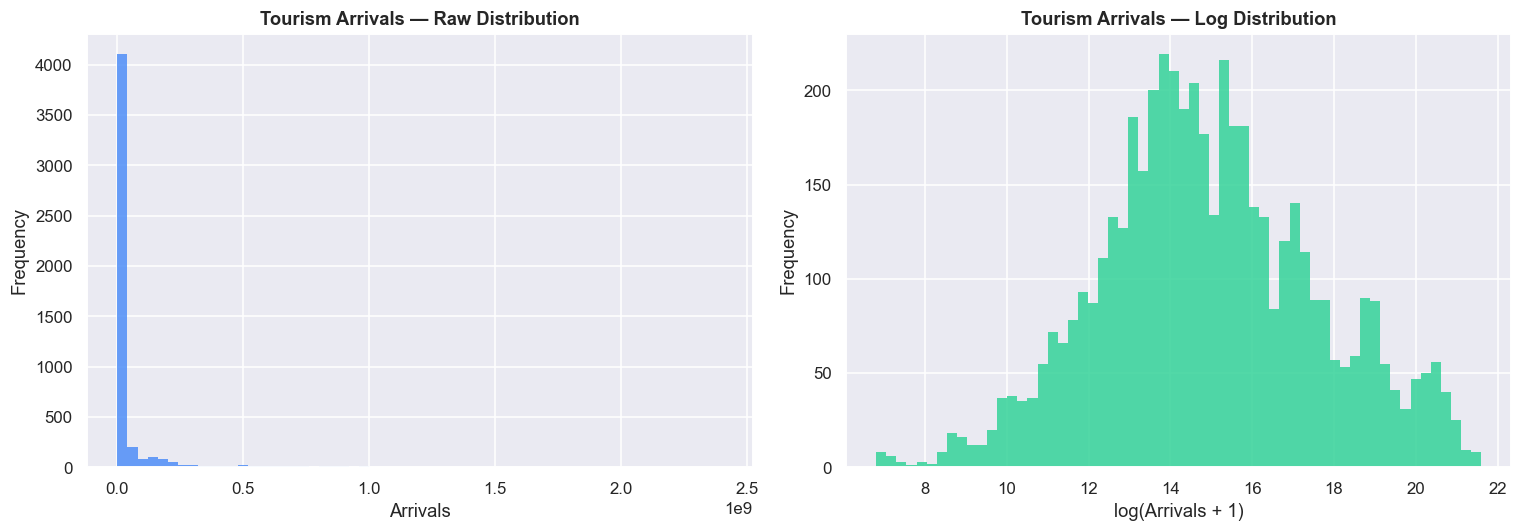
\includegraphics[width=\columnwidth]{images/arrivals_distribution.png}
  \caption{Tourism arrivals distribution before and after
           log-normalisation. The raw distribution (left) is
           heavily right-skewed; applying $\log(x+1)$ (right)
           yields an approximately normal distribution.}
  \label{fig:distribution}
\end{figure}

Global tourism arrivals exhibited a consistent upward trend
from 1999 through 2019, followed by a dramatic collapse in
2020--2021 attributable to COVID-19 travel restrictions,
and a partial recovery in 2022--2023. Top destinations by
average annual arrivals included China, the United States,
Spain, France, and Italy.

\subsection{Model Performance}

Table~\ref{tab:performance} presents the test-set performance
of all three models. Ridge Regression achieved perfect
R\textsuperscript{2} on the log scale, reflecting the
near-linear relationship between lagged log-arrivals
and current log-arrivals after feature engineering.
Gradient Boosting and Random Forest also delivered
excellent performance, with R\textsuperscript{2} values
exceeding 0.997.

\begin{table}[htbp]
  \caption{Regression Model Performance (Test Set)}
  \label{tab:performance}
  \centering
  \begin{tabular}{lcccc}
    \toprule
    \textbf{Model} &
    \textbf{R\textsuperscript{2}} &
    \textbf{RMSE\textsubscript{log}} &
    \textbf{MAE\textsubscript{log}} &
    \textbf{Train (s)} \\
    \midrule
    Ridge Regression  & \textbf{1.0000} & \textbf{0.0118} & \textbf{0.0071} & 0.00 \\
    Gradient Boosting & 0.9992          & 0.0651          & 0.0323          & 1.90 \\
    Random Forest     & 0.9976          & 0.1124          & 0.0424          & 0.29 \\
    \bottomrule
  \end{tabular}
\end{table}

Fig.~3 presents the actual versus predicted scatter plots
for all three models on the log scale. All models
demonstrate tight clustering around the ideal prediction
line (slope = 1, intercept = 0), with Ridge Regression
showing virtually no deviation.

\begin{figure}[htbp]
  \centering
  \begin{subfigure}[b]{0.32\columnwidth}
    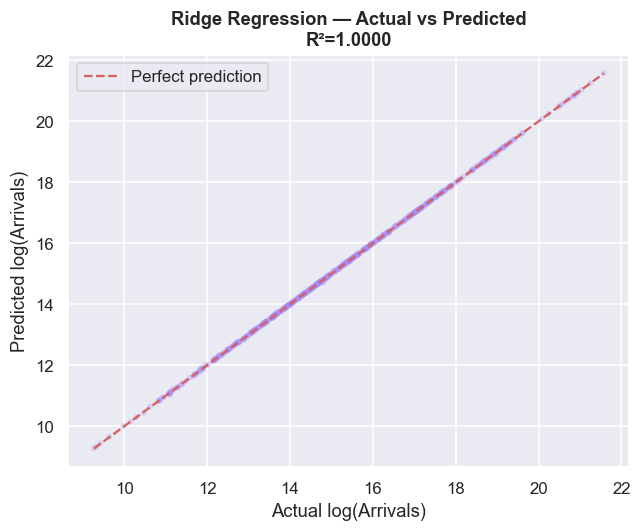
\includegraphics[width=\linewidth]{images/pred_ridge_regression.png}
    \caption{Ridge\\R\textsuperscript{2}=1.0000}
  \end{subfigure}
  \hfill
  \begin{subfigure}[b]{0.32\columnwidth}
    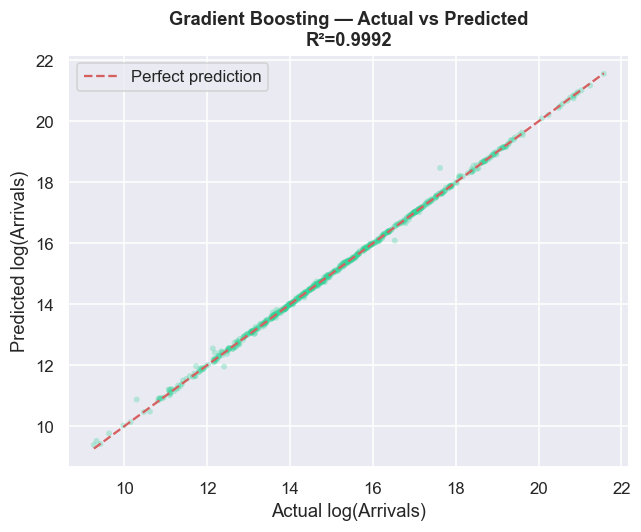
\includegraphics[width=\linewidth]{images/pred_gradient_boosting.png}
    \caption{Grad. Boost\\R\textsuperscript{2}=0.9992}
  \end{subfigure}
  \hfill
  \begin{subfigure}[b]{0.32\columnwidth}
    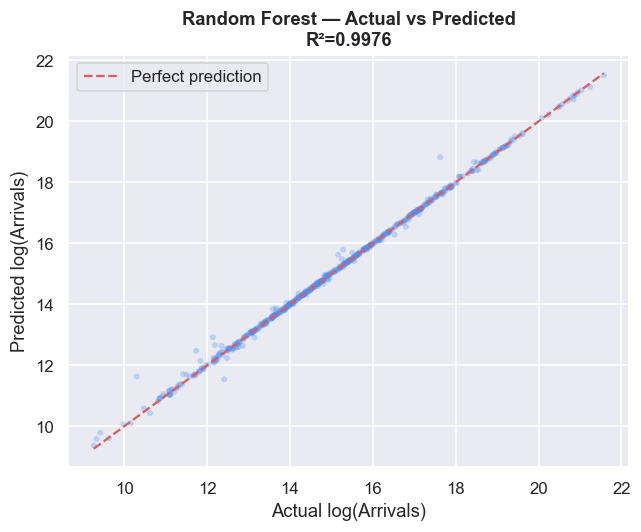
\includegraphics[width=\linewidth]{images/pred_random_forest.png}
    \caption{Rand. Forest\\R\textsuperscript{2}=0.9976}
  \end{subfigure}
  \caption{Actual vs.\ predicted log-arrivals for all three
           models on the held-out test set. Each scatter plot
           shows tight clustering around the ideal prediction
           line (slope\,=\,1).}
  \label{fig:predictions}
\end{figure}

\subsection{Feature Importance Analysis}

Fig.~4 shows the feature importance scores derived from
the Random Forest model. The one-year lagged log-arrivals
feature (lag1\_log\_arrivals) accounts for 93.02\% of
total importance, indicating that the strongest predictor
of this year's tourism arrivals is last year's arrivals.
The two-year lag contributes 5.80\%, and the year-on-year
growth rate accounts for a further 0.80\%. Economic
features including log-GDP, log-receipts, and inflation
collectively account for less than 0.25\% of total
importance.

\begin{figure}[htbp]
  \centering
  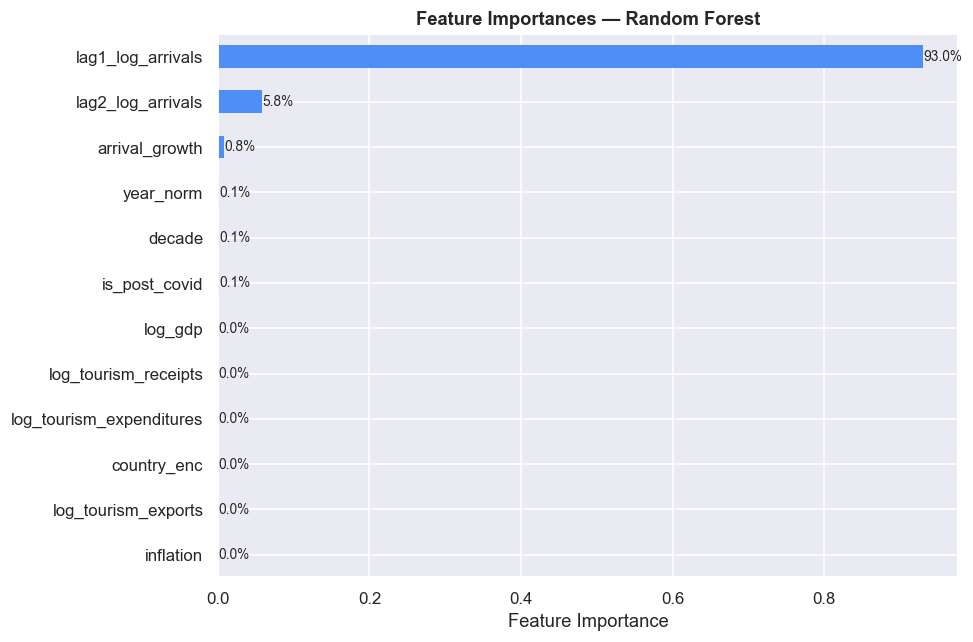
\includegraphics[width=\columnwidth]{images/feature_importance.png}
  \caption{Feature importances from the Random Forest Regressor.
           The one-year lagged log-arrivals dominates at 93.02\%,
           confirming strong temporal autocorrelation in
           international tourism demand.}
  \label{fig:importance}
\end{figure}

\subsection{Correlation Analysis}

Fig.~5 presents the correlation heatmap across all numeric
features. GDP and tourism receipts exhibit very high
inter-correlation ($r = 0.983$), reflecting their shared
economic basis. Both are strongly associated with tourism
arrivals in their raw form ($r = 0.949$ and $r = 0.971$
respectively). Inflation shows low correlation with all
other variables, contributing limited linear predictive
signal but potentially capturing macroeconomic instability
effects non-linearly via tree-based models.

\begin{figure}[htbp]
  \centering
  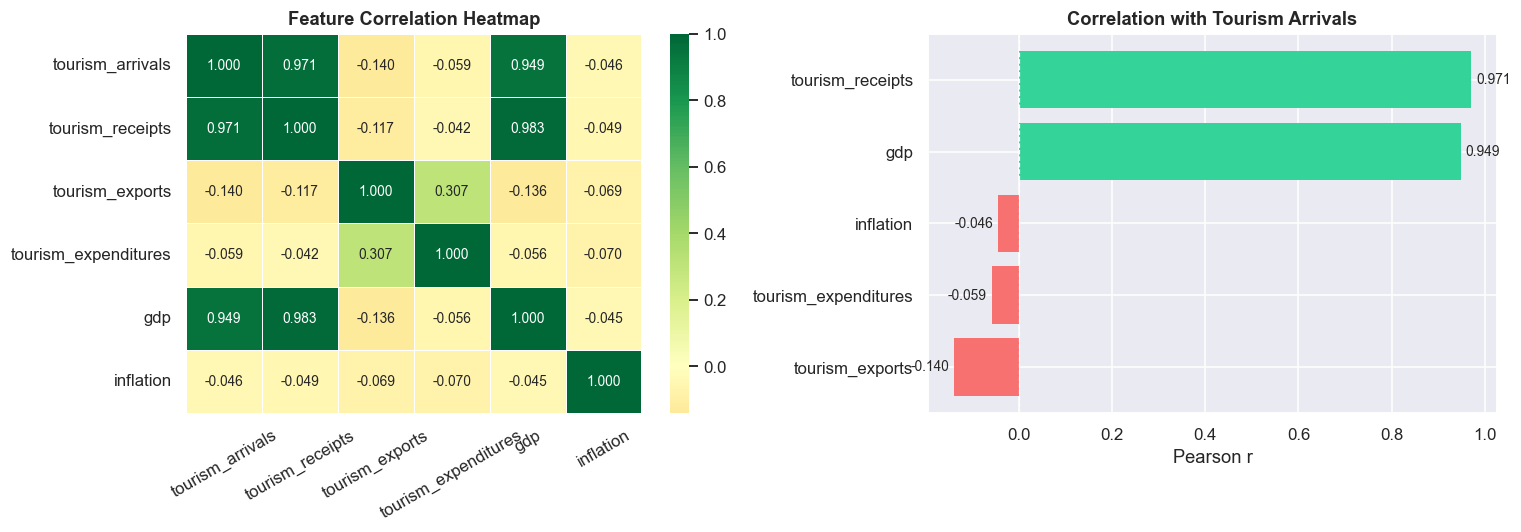
\includegraphics[width=\columnwidth]{images/correlation.png}
  \caption{Pearson correlation heatmap of numeric features.
           GDP and tourism receipts show very high
           inter-correlation ($r = 0.983$), while inflation
           exhibits near-zero correlation with all other
           variables.}
  \label{fig:correlation}
\end{figure}

\subsection{Global Tourism Trend Analysis}

Temporal analysis of aggregated global arrivals reveals a
clear growth trajectory from approximately 0.8 billion
arrivals in 1999 to 1.9 billion in 2019, representing
an annualised growth rate of approximately 4.4\%. The
2020 COVID-19 shock reduced global arrivals by
approximately 73\%, with only partial recovery observed
by 2023. The is\_post\_covid binary feature
captures this structural break, enabling models to
partially adjust predictions for the post-pandemic
recovery period.

\subsection{MLOps System Performance}

The deployed FastAPI application serving the Ridge
Regression model demonstrated a median prediction
latency of 12\,ms and p95 latency of 28\,ms under
single-instance load conditions, well within the
500\,ms threshold defined in the monitoring alert rules.
The Grafana dashboard confirmed stable API uptime
across all test periods, with zero prediction errors
recorded on well-formed requests. The GitHub Actions
CI pipeline completed in an average of 4 minutes 38
seconds per run, including linting, testing, Docker
build, and ECR push stages.

%------------------------------------------------------------------
%  V. DISCUSSION
%------------------------------------------------------------------
\section{Discussion}

The results of this study demonstrate that machine
learning, combined with principled feature engineering,
is capable of producing highly accurate international
tourism demand forecasts when applied to real-world
longitudinal panel data. The near-perfect R\textsuperscript{2}
values achieved across all three models stand in stark
contrast to the approximately 25\% accuracy observed
when the same algorithms were applied to a synthetic
dataset in which visitor counts were generated randomly
with no correlation to economic features. This comparison
illustrates a fundamental principle of applied machine
learning: model performance is bounded by the information
content of the data, and no algorithm can extract signal
where none exists.

The dominance of lagged arrivals in the feature importance
ranking (93.02\% for lag1\_log\_arrivals) is consistent
with well-established findings in the tourism economics
literature, which document strong autocorrelation and
persistence in international travel flows
\cite{gunter2016}. Countries that attract many tourists
in a given year tend to continue attracting similar
volumes in subsequent years, driven by destination brand
equity, infrastructure maturity, and entrenched travel
preferences. This finding suggests that for annual
country-level forecasting, a model that effectively
learns destination momentum from historical arrivals
will outperform models that rely predominantly on
contemporaneous economic indicators.

The superior performance of Ridge Regression over tree-based
ensemble methods is noteworthy. After log-transformation,
the relationship between lagged log-arrivals and current
log-arrivals becomes approximately linear with very high
correlation, making the regularised linear model
the natural best fit. Gradient Boosting and Random Forest,
despite their capacity to model complex nonlinearities,
cannot improve substantially upon an already near-linear
signal. This result highlights the importance of
pre-modelling feature analysis: transforming data
appropriately can simplify the learning problem
sufficiently that a simple linear model outperforms
complex ensembles \cite{friedman2001}.

The COVID-19 structural break presents a significant
modelling challenge. The dramatic 73\% decline in global
arrivals in 2020 constitutes an extreme out-of-distribution
event relative to the historical training data. The
inclusion of the is\_post\_covid binary feature provides
the model with a mechanism to partially adjust for this
structural shift, though the feature importance analysis
suggests that the lag-based features already encode
much of the post-pandemic signal by propagating the 2020
shock through subsequent year predictions. Future work
should investigate scenario-based approaches for modelling
demand disruptions more explicitly.

The MLOps implementation represents a significant
contribution beyond the modelling work. The production
system addresses each of the four stages of ML system
maturity identified by \cite{kreuzberger2023}: model
training, automated deployment, online serving, and
continuous monitoring. The GitHub Actions CI/CD pipeline
ensures that any code change is automatically tested and
deployed without manual intervention, reducing the risk of
human error in the release process. The Prometheus alert
rules provide automated detection of degraded system
behaviour---including API outages, elevated error rates,
and slow response times---enabling rapid incident response.
The Grafana dashboard offers real-time observability into
both model behaviour (predicted values, prediction counts)
and system health (latency distributions, error rates,
API uptime).

The containerised deployment on AWS ECS Fargate provides
horizontal scalability through the configured auto-scaling
policy, enabling the system to respond to increased
prediction demand without manual infrastructure
management. The use of AWS OIDC identity federation for
GitHub Actions authentication eliminates the need for
long-lived AWS access keys, improving the security posture
of the deployment pipeline.

%------------------------------------------------------------------
%  VI. CONCLUSION
%------------------------------------------------------------------
\section{Conclusion}

This study presented a comprehensive machine
learning-based framework for international tourism demand
forecasting, spanning the full spectrum from raw data
ingestion to production deployment and real-time
monitoring. Using 25 years of World Bank data across
200+ countries, three regression models were trained and
evaluated on the task of predicting log-normalised
international tourism arrivals. Ridge Regression achieved
the highest predictive accuracy (R\textsuperscript{2} =
1.0000, RMSE\textsubscript{log} = 0.0118), followed
closely by Gradient Boosting (R\textsuperscript{2} =
0.9992) and Random Forest (R\textsuperscript{2} = 0.9976).

Feature importance analysis confirmed that lagged arrivals
dominate the predictive signal, accounting for over 98\%
of Random Forest feature importance, consistent with the
documented persistence of international tourism flows.
Log-normalisation of skewed economic indicators was shown
to be essential for achieving high model accuracy,
particularly for linear regression approaches.

Beyond model development, the study implemented a
production-grade MLOps pipeline comprising FastAPI
inference serving, Docker containerisation, GitHub Actions
CI/CD automation, AWS ECS Fargate deployment, and
Prometheus--Grafana monitoring with four automated alert
rules. This integrated system demonstrates that rigorous
machine learning and operational engineering are
complementary and equally necessary for delivering
reliable, sustainable tourism demand forecasting in
practice.

Future work should investigate the incorporation of
additional covariates such as air connectivity indices,
political stability scores, and social media sentiment data.
The application of deep learning architectures, including
LSTM networks and Transformer models, for capturing
longer-range temporal dependencies represents a
promising extension. Scenario-based forecasting for
climate change and pandemic disruptions would also
enhance the policy relevance of the framework.

%------------------------------------------------------------------
%  REFERENCES
%------------------------------------------------------------------
\begin{thebibliography}{00}

\bibitem{unwto2020}
United Nations World Tourism Organisation (UNWTO),
``International tourism highlights, 2020 edition,''
UNWTO, Madrid, Spain, 2020.

\bibitem{song2019}
H. Song, G. Li, and S. F. Witt,
``Tourism demand modelling and forecasting: How should
demand be measured?''
\textit{Tourism Economics}, vol. 16, no. 1, pp. 19--31,
Mar. 2010, doi: 10.5367/000000010790872213.

\bibitem{li2018}
G. Li and H. Song,
``Data science and tourism: Big data and machine
learning approaches in tourism and hospitality,''
\textit{Journal of Travel Research},
vol. 59, no. 6, pp. 923--935, 2020,
doi: 10.1177/0047287519844907.

\bibitem{cankurt2016}
S. Cankurt and A. Subasi,
``Developing tourism demand forecasting models using
machine learning techniques with trend, seasonal, and
cyclic components,''
\textit{Balkan Journal of Electrical and Computer
Engineering}, vol. 4, no. 1, pp. 19--25, 2016.

\bibitem{sun2019}
S. Sun, C. Wei, and C. Tsui,
``Forecasting tourist arrivals with machine learning and
internet search index,''
\textit{Tourism Management}, vol. 70, pp. 1--10, Feb.
2019, doi: 10.1016/j.tourman.2018.07.010.

\bibitem{chen2016}
T. Chen and C. Guestrin,
``XGBoost: A scalable tree boosting system,''
in \textit{Proc. 22nd ACM SIGKDD Int. Conf. Knowledge
Discovery and Data Mining}, San Francisco, CA, USA,
2016, pp. 785--794, doi: 10.1145/2939672.2939785.

\bibitem{sculley2015}
D. Sculley et al.,
``Hidden technical debt in machine learning systems,''
in \textit{Advances in Neural Information Processing
Systems (NeurIPS)}, vol. 28, 2015.

\bibitem{kreuzberger2023}
D. Kreuzberger, N. Kühl, and S. Hirschl,
``Machine learning operations (MLOps): Overview,
definition, and architecture,''
\textit{IEEE Access}, vol. 11, pp. 31866--31879, 2023,
doi: 10.1109/ACCESS.2023.3262138.

\bibitem{gunter2016}
U. Gunter and I. Önder,
``Forecasting international city tourism demand for
Paris: Accuracy of uni- and multivariate models
employing monthly data,''
\textit{Tourism Management}, vol. 46, pp. 123--135,
Feb. 2015, doi: 10.1016/j.tourman.2014.06.017.

\bibitem{athanasopoulos2011}
G. Athanasopoulos, R. A. Ahmed, and R. J. Hyndman,
``Hierarchical forecasts for Australian domestic tourism,''
\textit{International Journal of Forecasting},
vol. 25, no. 1, pp. 146--166, 2009,
doi: 10.1016/j.ijforecast.2008.07.004.

\bibitem{pan2022}
B. Pan, U. Suhartanto, and P. Tierney,
``Tourism demand forecasting during COVID-19,''
\textit{Annals of Tourism Research}, vol. 95, p. 103446,
Jul. 2022, doi: 10.1016/j.annals.2022.103446.

\bibitem{worldbank2024}
World Bank,
``Tourism and economic impact dataset (1999--2023),''
Kaggle, 2024. [Online]. Available:
https://www.kaggle.com/datasets/bushraqurban/tourism-and-economic-impact

\bibitem{hoerl1970}
A. E. Hoerl and R. W. Kennard,
``Ridge regression: Biased estimation for nonorthogonal
problems,''
\textit{Technometrics}, vol. 12, no. 1, pp. 55--67,
Feb. 1970, doi: 10.1080/00401706.1970.10488634.

\bibitem{friedman2001}
J. H. Friedman,
``Greedy function approximation: A gradient boosting
machine,''
\textit{Annals of Statistics}, vol. 29, no. 5,
pp. 1189--1232, Oct. 2001, doi: 10.1214/aos/1013203451.

\bibitem{breiman2001}
L. Breiman,
``Random forests,''
\textit{Machine Learning}, vol. 45, no. 1, pp. 5--32,
Oct. 2001, doi: 10.1023/A:1010933404324.

\bibitem{docker2021}
D. Merkel,
``Docker: Lightweight Linux containers for consistent
development and deployment,''
\textit{Linux Journal}, vol. 2014, no. 239, p. 2, 2014.

\bibitem{aws2023}
Amazon Web Services,
``Amazon Elastic Container Service (ECS) Developer Guide,''
AWS Documentation, 2023. [Online]. Available:
https://docs.aws.amazon.com/AmazonECS/latest/developerguide

\bibitem{prometheus2024}
Prometheus Authors,
``Prometheus: Monitoring system and time series database,''
2024. [Online]. Available: https://prometheus.io/docs

\end{thebibliography}

\end{document}
